\apendice{Documentación de usuario}

\section{Introducción}
En este punto de procederá a explicar el manual del usuario para el uso de la aplicación. Las indicaciones se hacen sobre un sistema \textit{Windows}, pero al ser una aplicación web, con tener instalado el buscador \textit{Chrome} en su última versión, servirá para poder interactuar con el sistema.

\section{Requisitos de usuarios}
Los requisitos para los usuarios son muy simples, al ser una aplicación web, funcionaria en cualquier buscador, pero se recomienda:
\begin{itemize}
    \item Ordenador, tablet o dispositivo móvil con mínimo 2 GB de memoria \textit{RAM}.
    \item Buscador \textit{Chrome} en versión 88.0 o superior.
\end{itemize}
\section{Instalación}
Al ser una aplicación web, no requiere de instalaciones extra para poder funcionar, lo que si es necesario es el despliegue de placas \textit{UWB} y las \textit{Raspberries} necesarias para que el sistema funcione.

\section{Manual del usuario}
\subsection{Usuario}
El usuario tiene diversas funcionalidades. Al entrar se encuentra en la pagina de \textit{Login}.
\FloatBarrier
\begin{figure}[h]
    \centering
    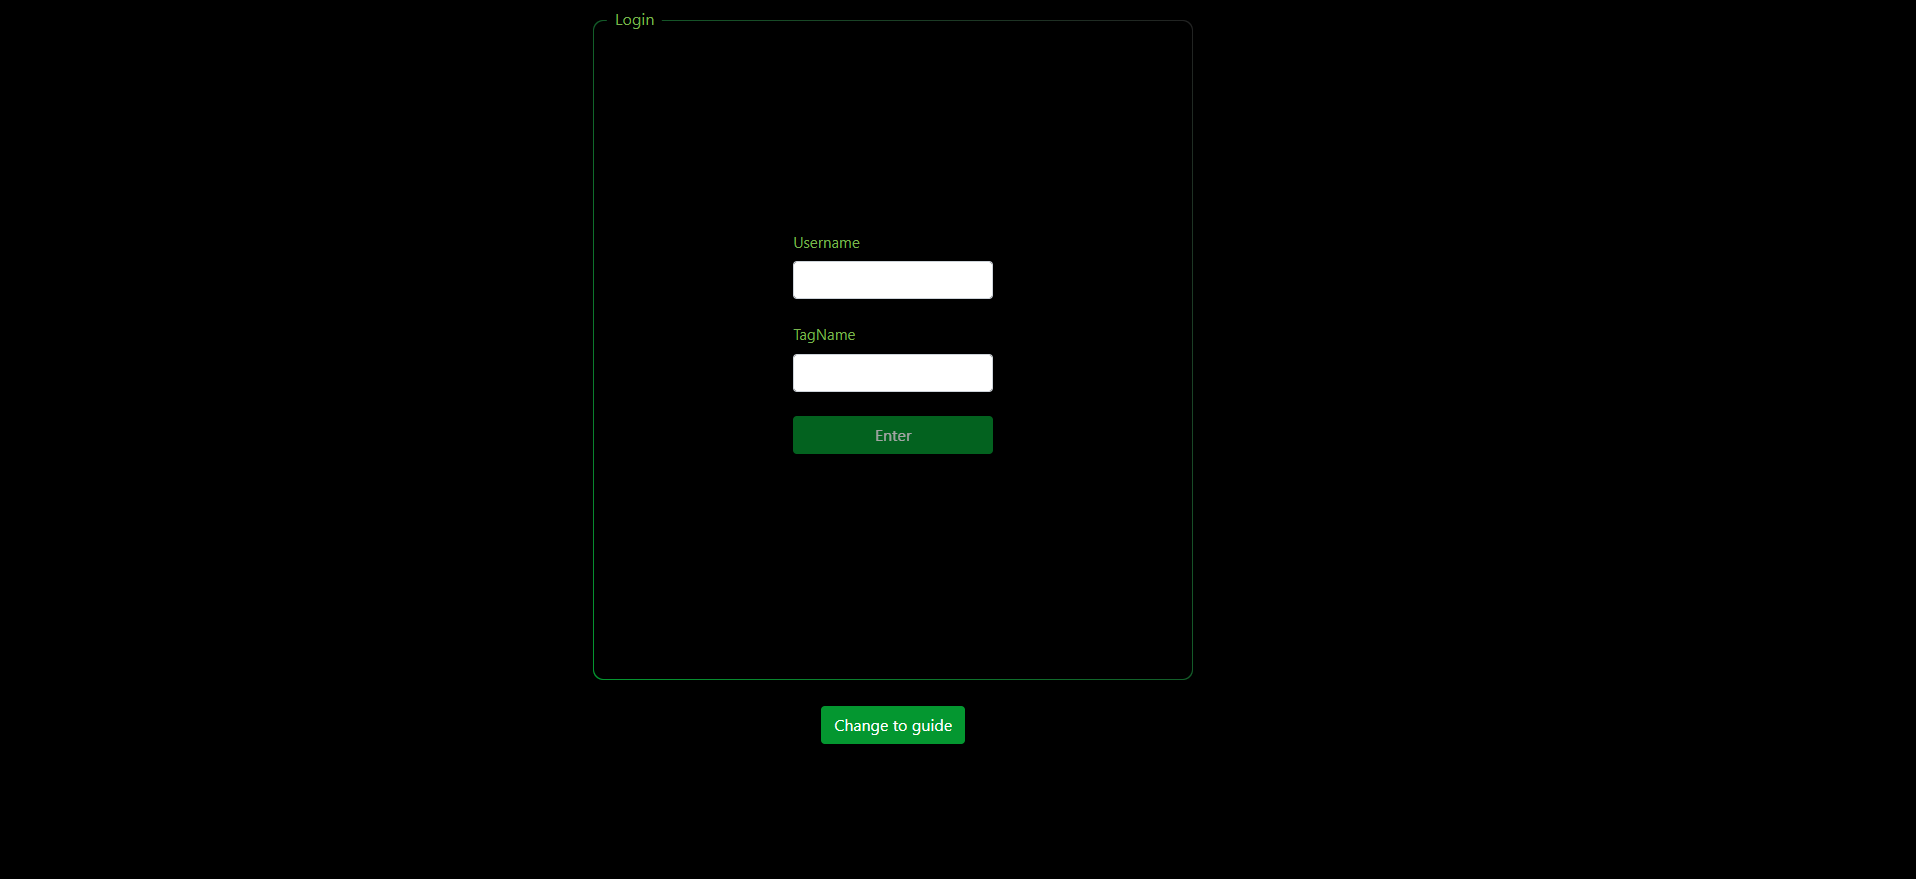
\includegraphics[width=10cm,height=10cm,keepaspectratio]{img/Login.png}
    \caption{Página de \textit{Login en la vista Usuario}.}
    \label{fig:Página de Login en la vista Usuario}
\end{figure}
\FloatBarrier

Una vez hace el \textit{Login} correctamente y se le enlaza con una \textit{Tag} pasa a la página del \textit{chat}, donde se le asigna una visita, y comparte vídeo y audio.


La aplicación tendrá acceso a la cámara y se podrán identificar obras de arte. Pudiendo recibir del guía las indicaciones pintadas sobre una capa \textit{canvas} sobre la obra de arte. Como último paso se podrá hacer logout, quitando en enlace usuario-tag de la base de datos.
\FloatBarrier
\begin{figure}[h]
    \centering
    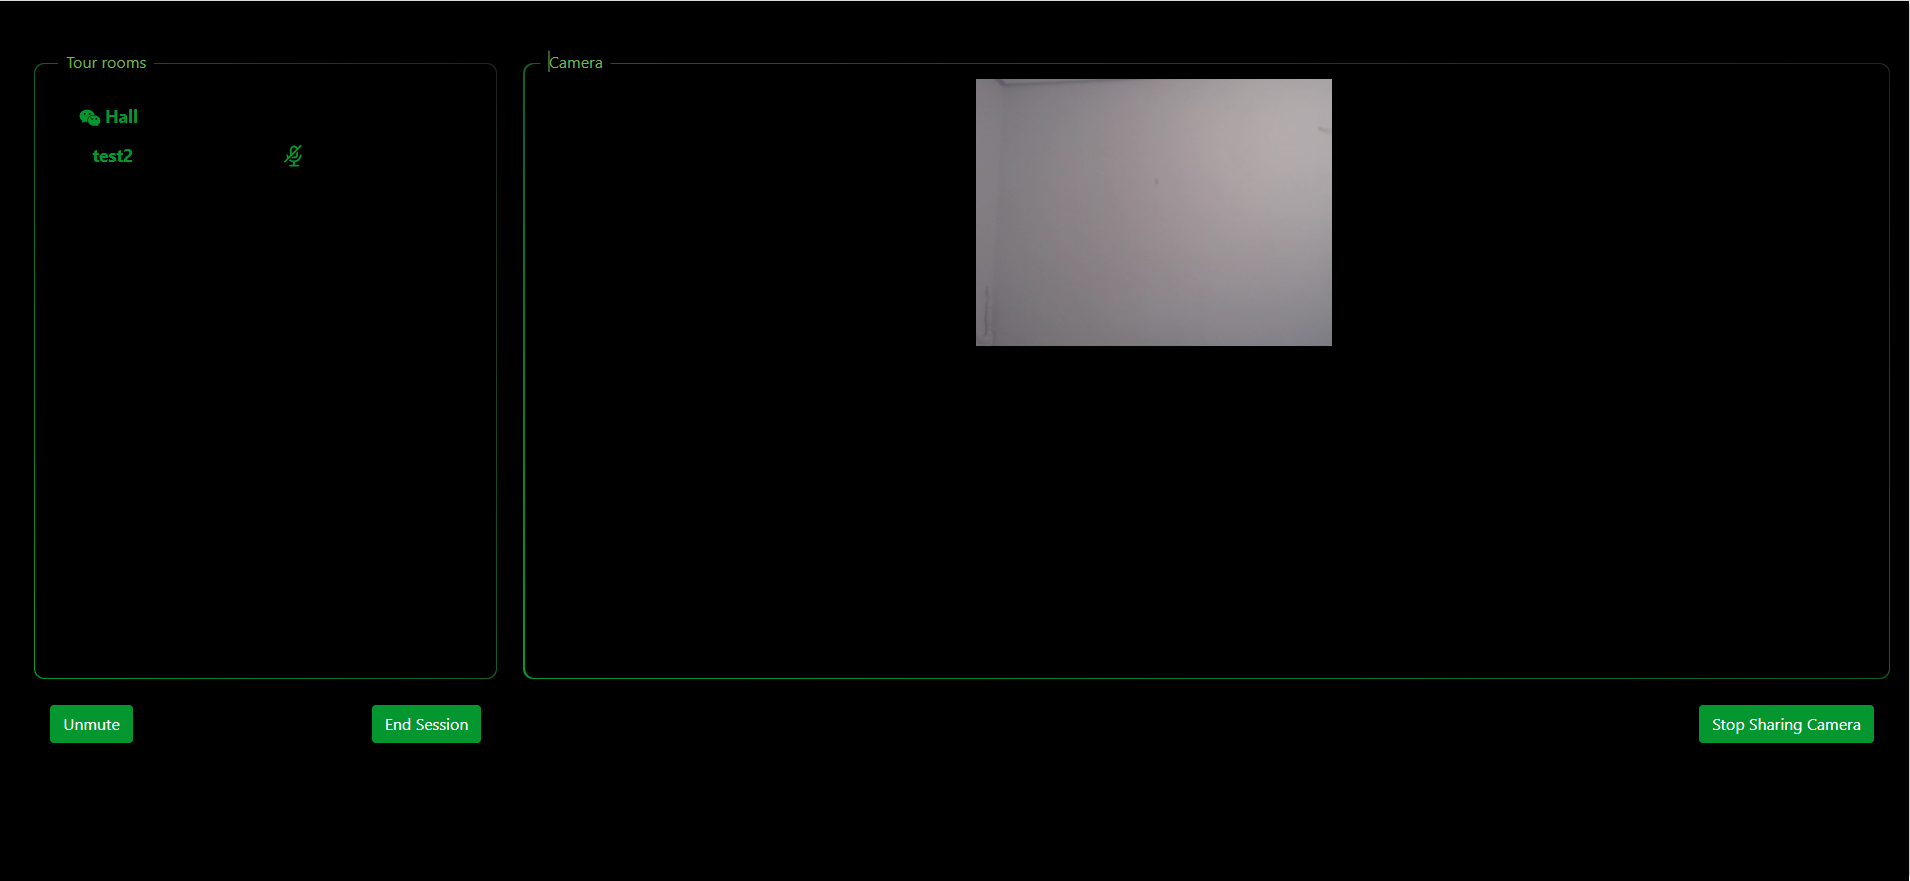
\includegraphics[width=10cm,height=10cm,keepaspectratio]{img/UserChatDesktop.png}
    \caption{Página chat desde la visión de usuario.}
    \label{fig:Página chat desde la visión de usuario}
\end{figure}
\FloatBarrier

Esta pagina de \textit{chat} cuenta con un diseños para ser visualizados desde múltiples dispositivos, diseños \textit{responsives}, ya que están pensados para ser usado por el usuario desde una \textit{tablet} o un dispositivo móvil.
\FloatBarrier
\begin{figure}[h]
    \centering
    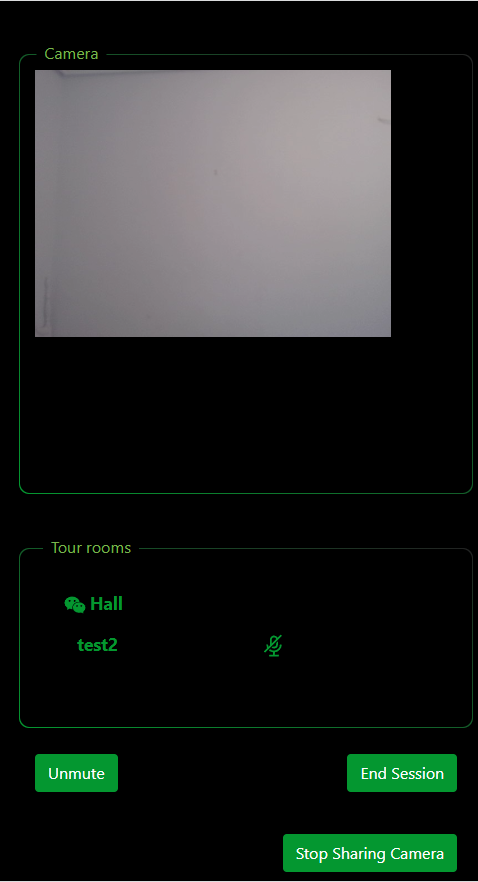
\includegraphics[width=10cm,height=10cm,keepaspectratio]{img/UserChatMobile.png}
    \caption{Página de chat desde la visión de un usuario con un dispositivo móvil.}
    \label{fig:diagram_seceunce_guide}
\end{figure}
\FloatBarrier
\subsection{Guía}

El usuario guia ha de hacer \textit{login} con un nombre especifico, si se hace correctamente se pasará a la sala del \textit{chat}.
\FloatBarrier
\begin{figure}[h]
    \centering
    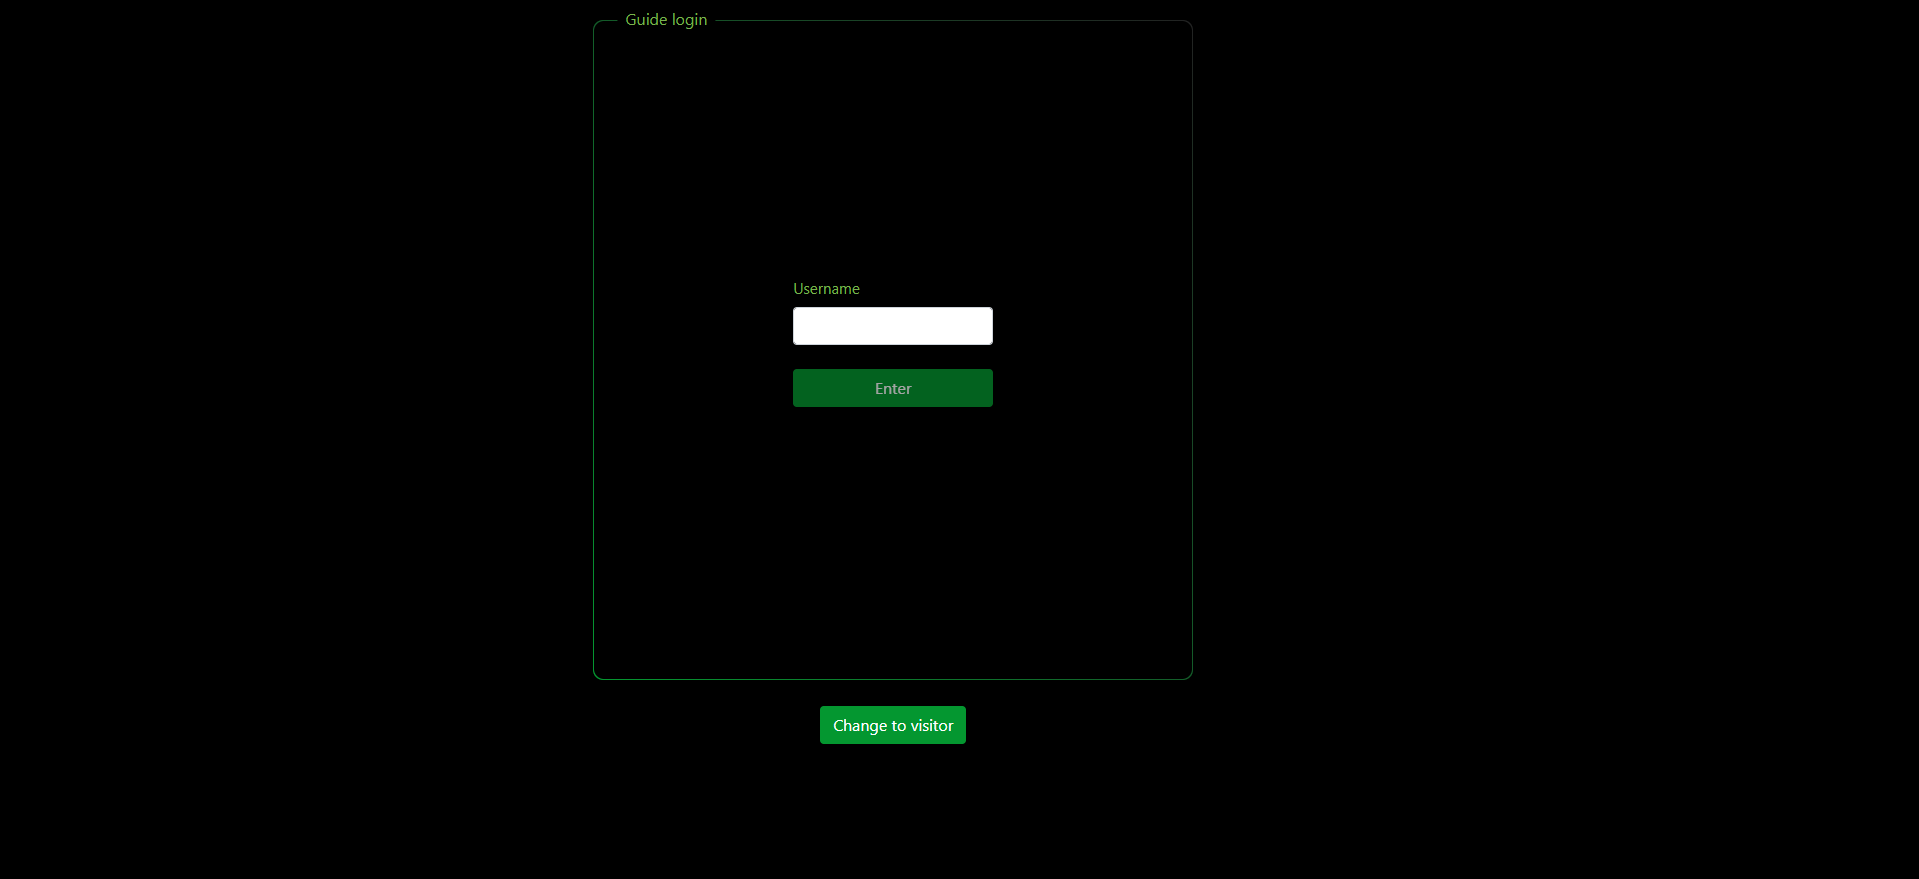
\includegraphics[width=10cm,height=10cm,keepaspectratio]{img/LoginGuide.png}
    \caption{Página \textit{Login} desde la visión del guía.}
    \label{fig:diagram_seceunce_guide}
\end{figure}
\FloatBarrier
En esta sala se tendrá una visión general de los usuarios en las visitas, hay una característica de \textit{drag and drop} que permite meter y sacar usuarios de tours arrastrándolos y soltándolos.


Además se podrán ver las cámaras y audio, teniendo control por separado, de hasta 4 usuarios simultáneamente. Se podrá ir desde un botón a la página de mapa.
\FloatBarrier
\begin{figure}[h]
    \centering
    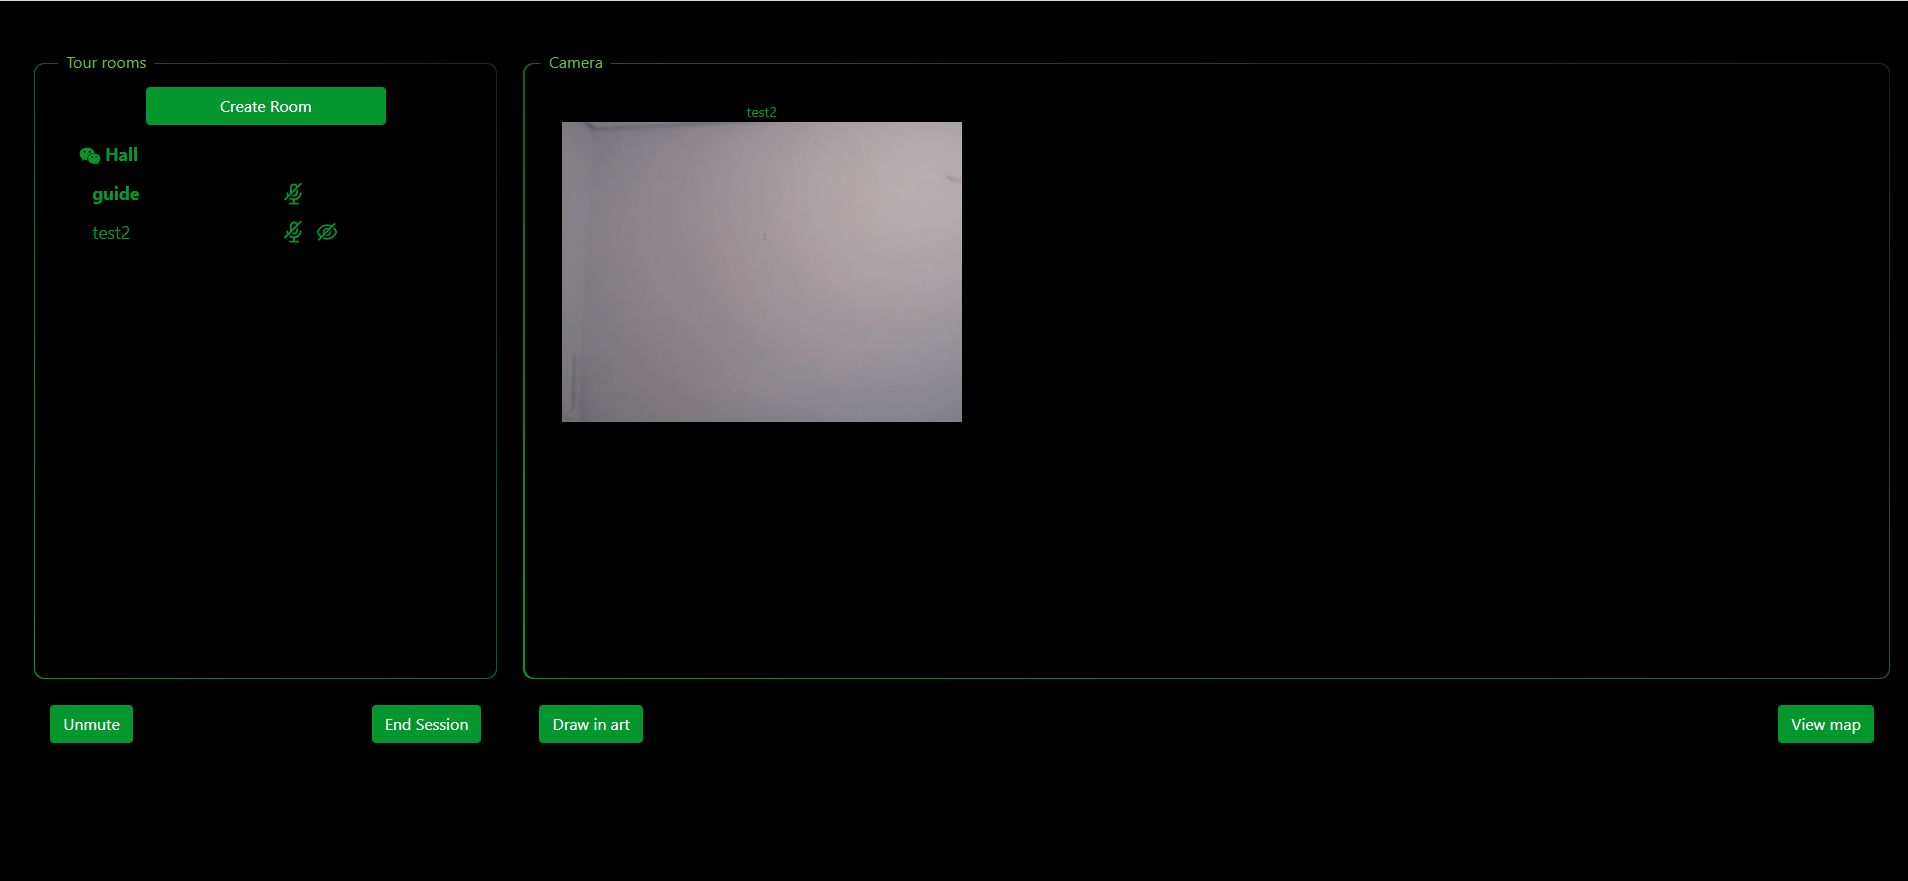
\includegraphics[width=10cm,height=10cm,keepaspectratio]{img/GuideChatDesktop.png}
    \caption{Página \textit{chat} desde la visión del guía.}
    \label{fig:diagram_seceunce_guide}
\end{figure}
\FloatBarrier

En la pagina de mapa, tendremos un \textit{sidebar} con toda la información relevante de los \textit{Anchors}, \textit{Tags} y \textit{Rooms}. De fondo se verá el mapa con \textit{Anchors}, \textit{Tags} y \textit{Rooms} renderizado a tiempo real.

Además se puede pinchar sobre \textit{Anchors} y \textit{Tags}, dando información extra en un segundo \textit{sidebar}.
\FloatBarrier
\begin{figure}[h]
    \centering
    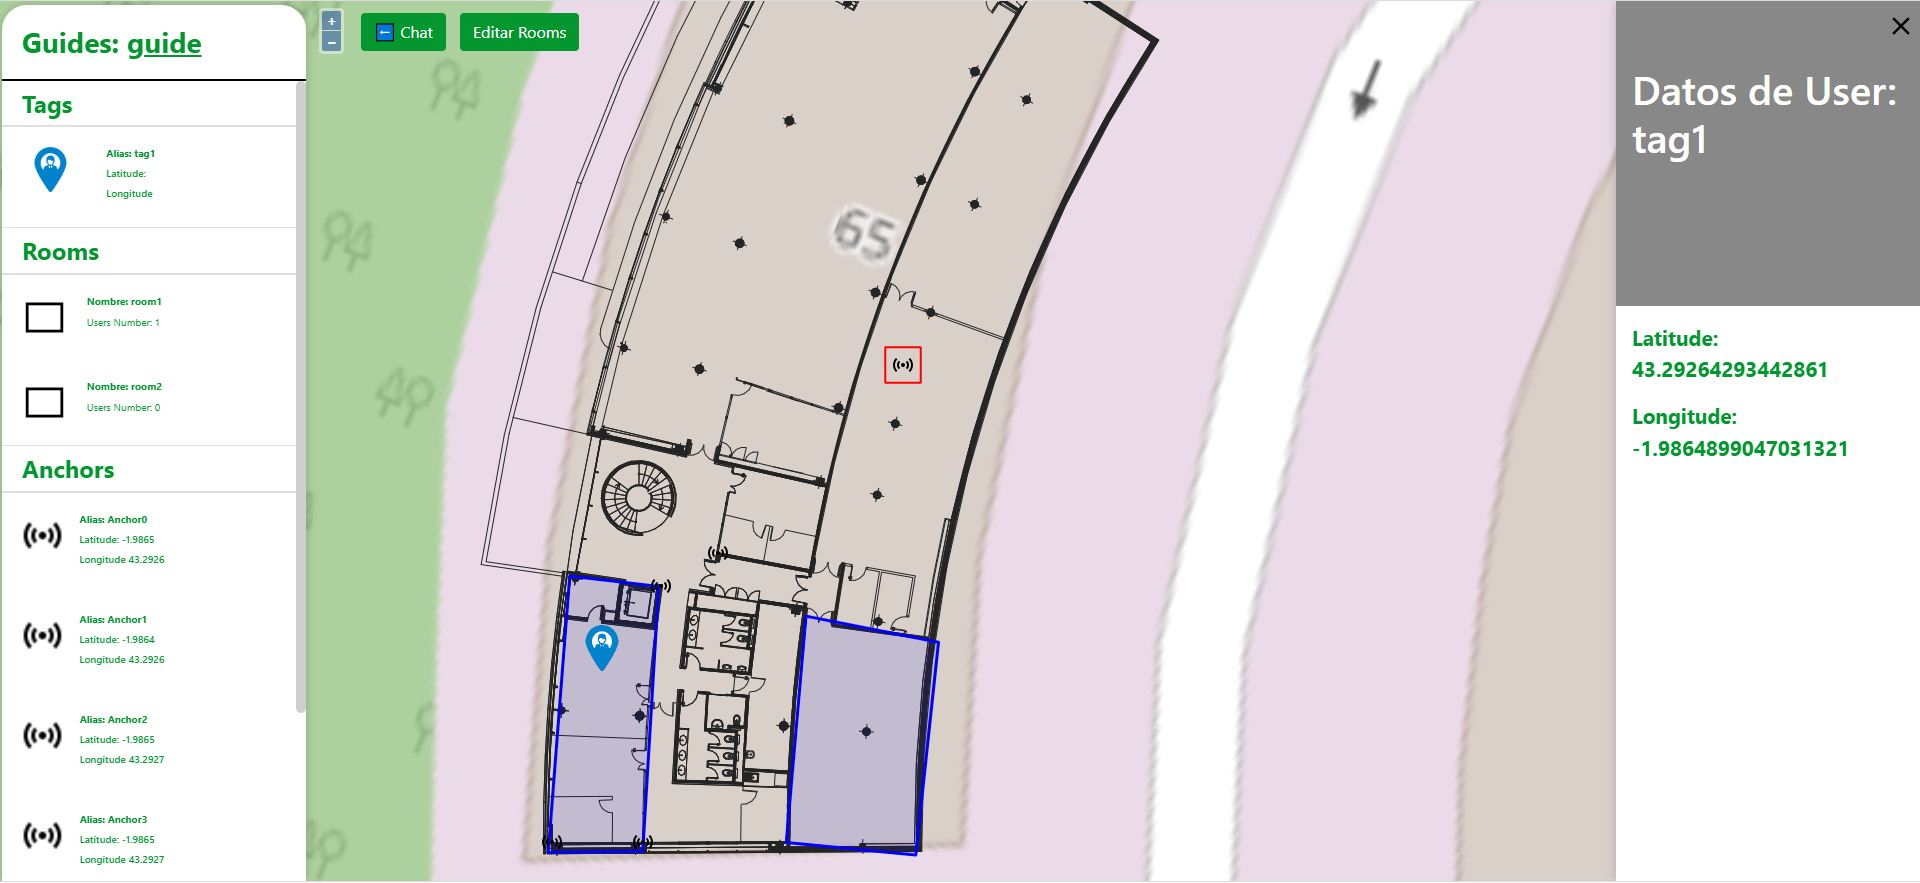
\includegraphics[width=10cm,height=10cm,keepaspectratio]{img/tagsidebar.png}
    \caption{Página Mapa con el \textit{sidebar} de visualización de un único \textit{Tag}.}
    \label{fig:diagram_seceunce_guide}
\end{figure}
\FloatBarrier

Si pinchamos sobre un \textit{Anchor}, en el segundo \textit{sidebar} se podrá permitir el movimiento del \textit{Anchor} arrastrándolo y soltándolo, persistiendo su nueva posición en la base de datos si así lo deseamos mediante el botón "Guardar Anchor" . 
\FloatBarrier
\begin{figure}[h]
    \centering
    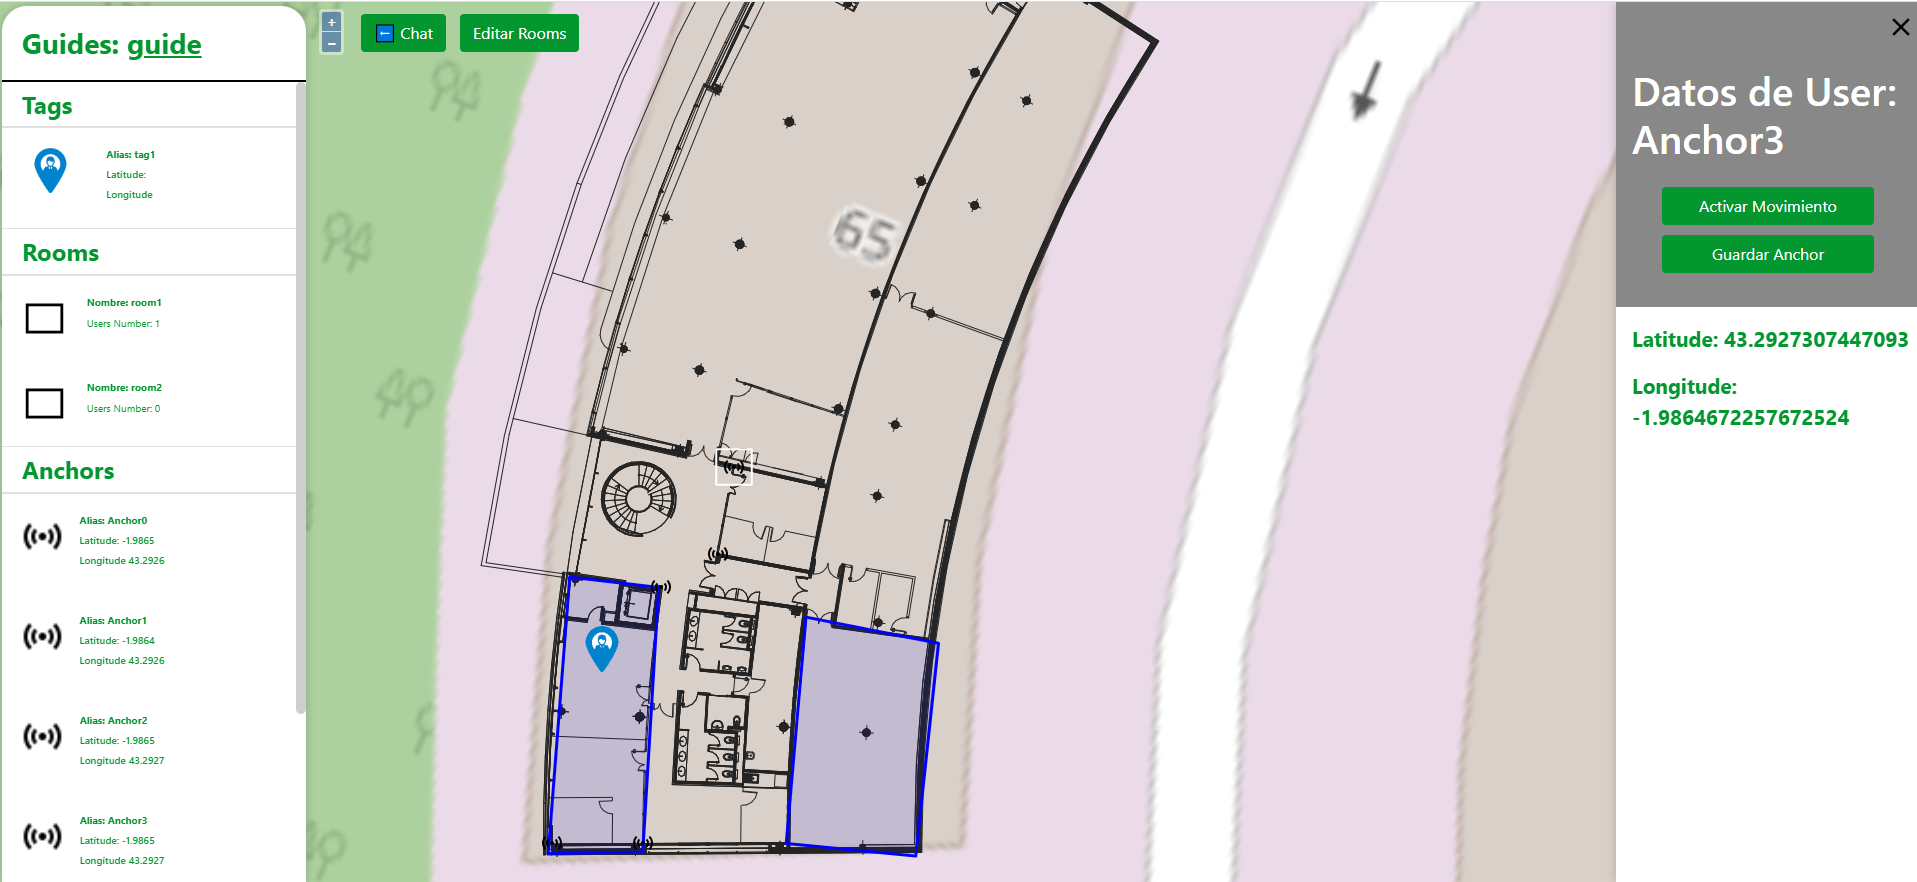
\includegraphics[width=10cm,height=10cm,keepaspectratio]{img/anchorsidebar.png}
    \caption{Página Mapa con el \textit{sidebar} de control de un \textit{Anchor}.}
    \label{fig:Página Mapa con el sidebar de control de un Anchor}
\end{figure}
\FloatBarrier
Si el \textit{Anchor} ha sido movido pero no guardado, saldrá un cuadrado rojo.
\FloatBarrier
\begin{figure}[h]
    \centering
    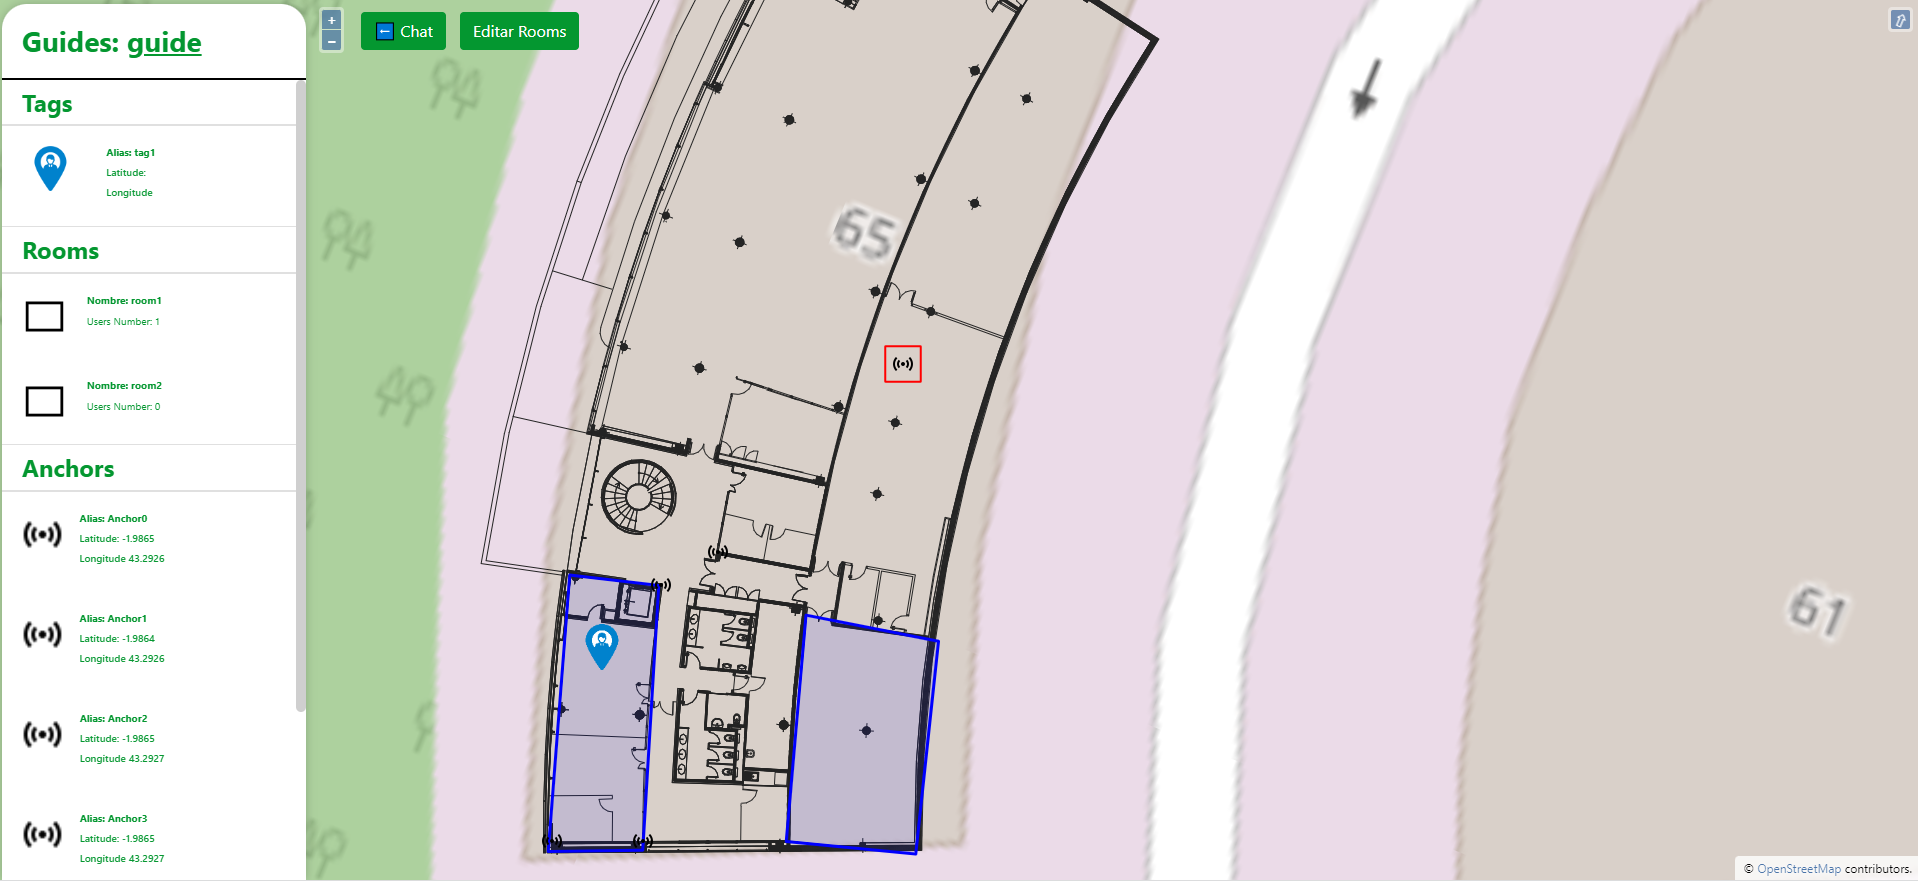
\includegraphics[width=10cm,height=10cm,keepaspectratio]{img/anchorsidebarMoved.png}
    \caption{Página Mapa gestionando la posición de un \textit{Anchor} sin guardar desde la vista del guía.}
    \label{fig:Página Mapa gestionando la posición de un Anchor sin guardar desde la vista del guía}
\end{figure}
\FloatBarrier

Desde la página de Mapa podemos ir a la página de EditarRoom, donde podemos crear y eliminar \textit{Rooms}.



La vista general es el mapa cargado solo con las \textit{Rooms} y un \textit{sidebar} con las \textit{Rooms} existentes y un botón para eliminar. Se podrán dibujar las \textit{Rooms} con el polígono que queramos y guardarlo en la base de datos, mediante el control de botones de la parte superior de la página.

\FloatBarrier
\begin{figure}[h]
    \centering
    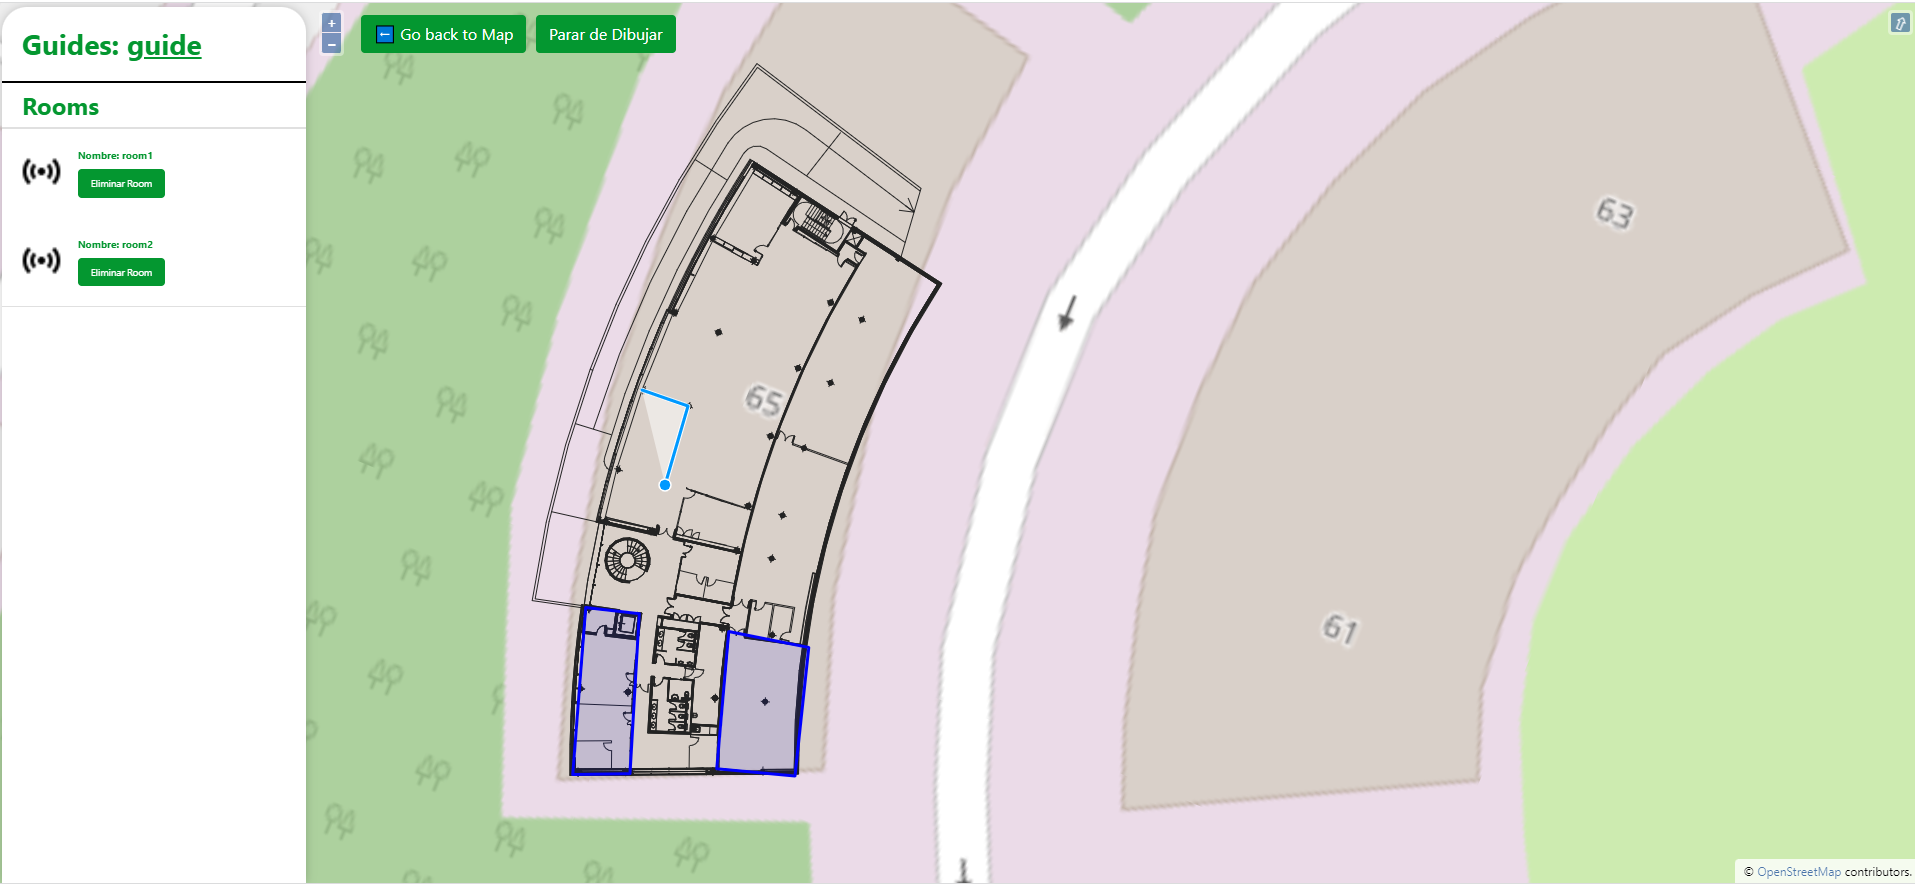
\includegraphics[width=10cm,height=10cm,keepaspectratio]{img/EditRoom.png}
    \caption{Página \textit{EditarRoom} de la vista del guía.}
    \label{fig:Página Editar Room de la vista del guía}
\end{figure}
\FloatBarrier


